\documentclass[11pt,draftclsnofoot,onecolumn,journal,letterpaper]{IEEEtran}
%\documentclass{IEEEtran}

\usepackage[UTF8]{ctex}
\begin{document}

\title{基于强化学习的无线网络自组织性研究}

\maketitle

%\begin{abstract}
%
%\end{abstract}

\section{引言}
%从5G的发展引入SON技术,并说明leaning算法的应用趋势
在5G系统中,移动通信面对更加多样化的业务需求和指标,5G 系统采用了更为复杂的无线传输技术和融合的无线网络架构,融合了多种接入方式、多种制式、多种架构的异构网络。超密集组网使得未来网络将进一步使现有的小区结构微型化、分布化 , 并加强小区间的相互协作;LTE、UMTS、WiFi等多种制式网络将在5G中共存;SDN/NFV等虚拟化架构引入到5G 当中,而更多密集的小型基站甚至支持“即插即用”等更加便捷智能的配置。因此,网络管理复杂度远远高于现有网络,网络深度智能化成为保证 5G 网络性能的迫切需要,使得更加智能的自组织网络(Self Organizing Network, SON)将成为 5G 不可或缺的又一关键技术。为了全面的了解SON的智能化发展现状,本文在强化学习算法在SON的技术方面的进展进行详细的研究。

\subsection{自组织网络简介}

%介绍无线自组织网络发展现状,以及部署在5G网络中的具体应用
%强调learning算法在SON中应用的必要性。

在传统的移动通信网络中,网络部署、运维等基本依靠人工的方式,需要投入大量的人力,给运营商带来巨大的运行成本。并且,随着移动通信网络的发展,依靠人工的方式难以实现网络的优化。因此,为了解决网络部署、优化的复杂性问题,降低运维成本相对总收入的比例,使运营商能高效运营、维护网络,在满足客户需求的同时,自身也能够持续发展,由 NGMN (Next Generation Mobile Network) 联盟中的运营商主导,联合主要的设备制造商提出了自组织网络 (SON) 的概念\cite{Alliance2008}。由于 5G 将采用大规模 MIMO 无线传输技术,使得空间自由度大幅度增加,从而带来天线选择、协作节点优化、波束选择、波束优化、多用户联合资源调配等方面的灵活性。对这些技术的优化,是5G 系统SON技术的重要内容。自组织网络的思路是在网络中引入自组织能力即实现网络智能化,包括自配置、自优化、自愈合等实现网络规划、部署、维护、优化和排障等各个环节的自动进行,最大限度地减少人工干预,并结合先进的学习理论逐步提升网络智能化。


\subsection{强化学习简介}

%简单概括强化学习定义,泛化介绍其特点,应用,不用展开,第二部分会具体讲
%介绍强化学习的发展现状,与通信场景结合实际应用的可行性分析。

SON在蜂窝网络中被定义为一个网络的概念,不仅具有自适应和自主功能,而且还具有足够的可扩展性,稳定性和灵活性,即使在环境发生变化时也能保持其期望的目标。虽然学习的方法没有直接包含在SON的定义中,但学习算法在系统功能的实现以及自动维护的问题上可以代替人工更有效地解决预料之外的问题。\emph{强化学习(Reinforcement Learning, RL)}是一种应用较为普遍的学习算法,这种算法以环境的状态作为输入,通过系统与环境的交互和试错,根据在交互过程中产生的评价性反馈信号,实现最终决策的不断优化。传统的有监督学习(Supervised Learning)依靠有标签的数据样本通过分类器推断功能,从而得到新实例的映射。无监督学习(Unsupervised Learning)相反是针对无标签数据进行自主结构性学习的过程。强化学习类似无监督学习,同样不需要预先标记的数据,不同的是强化学习依靠与环境及状态的实时信息交互,即从环境中获得回报(Reward)并依此调整策略,逐渐获得最大化的预期利益。
\begin{figure}%[h]
\centerline{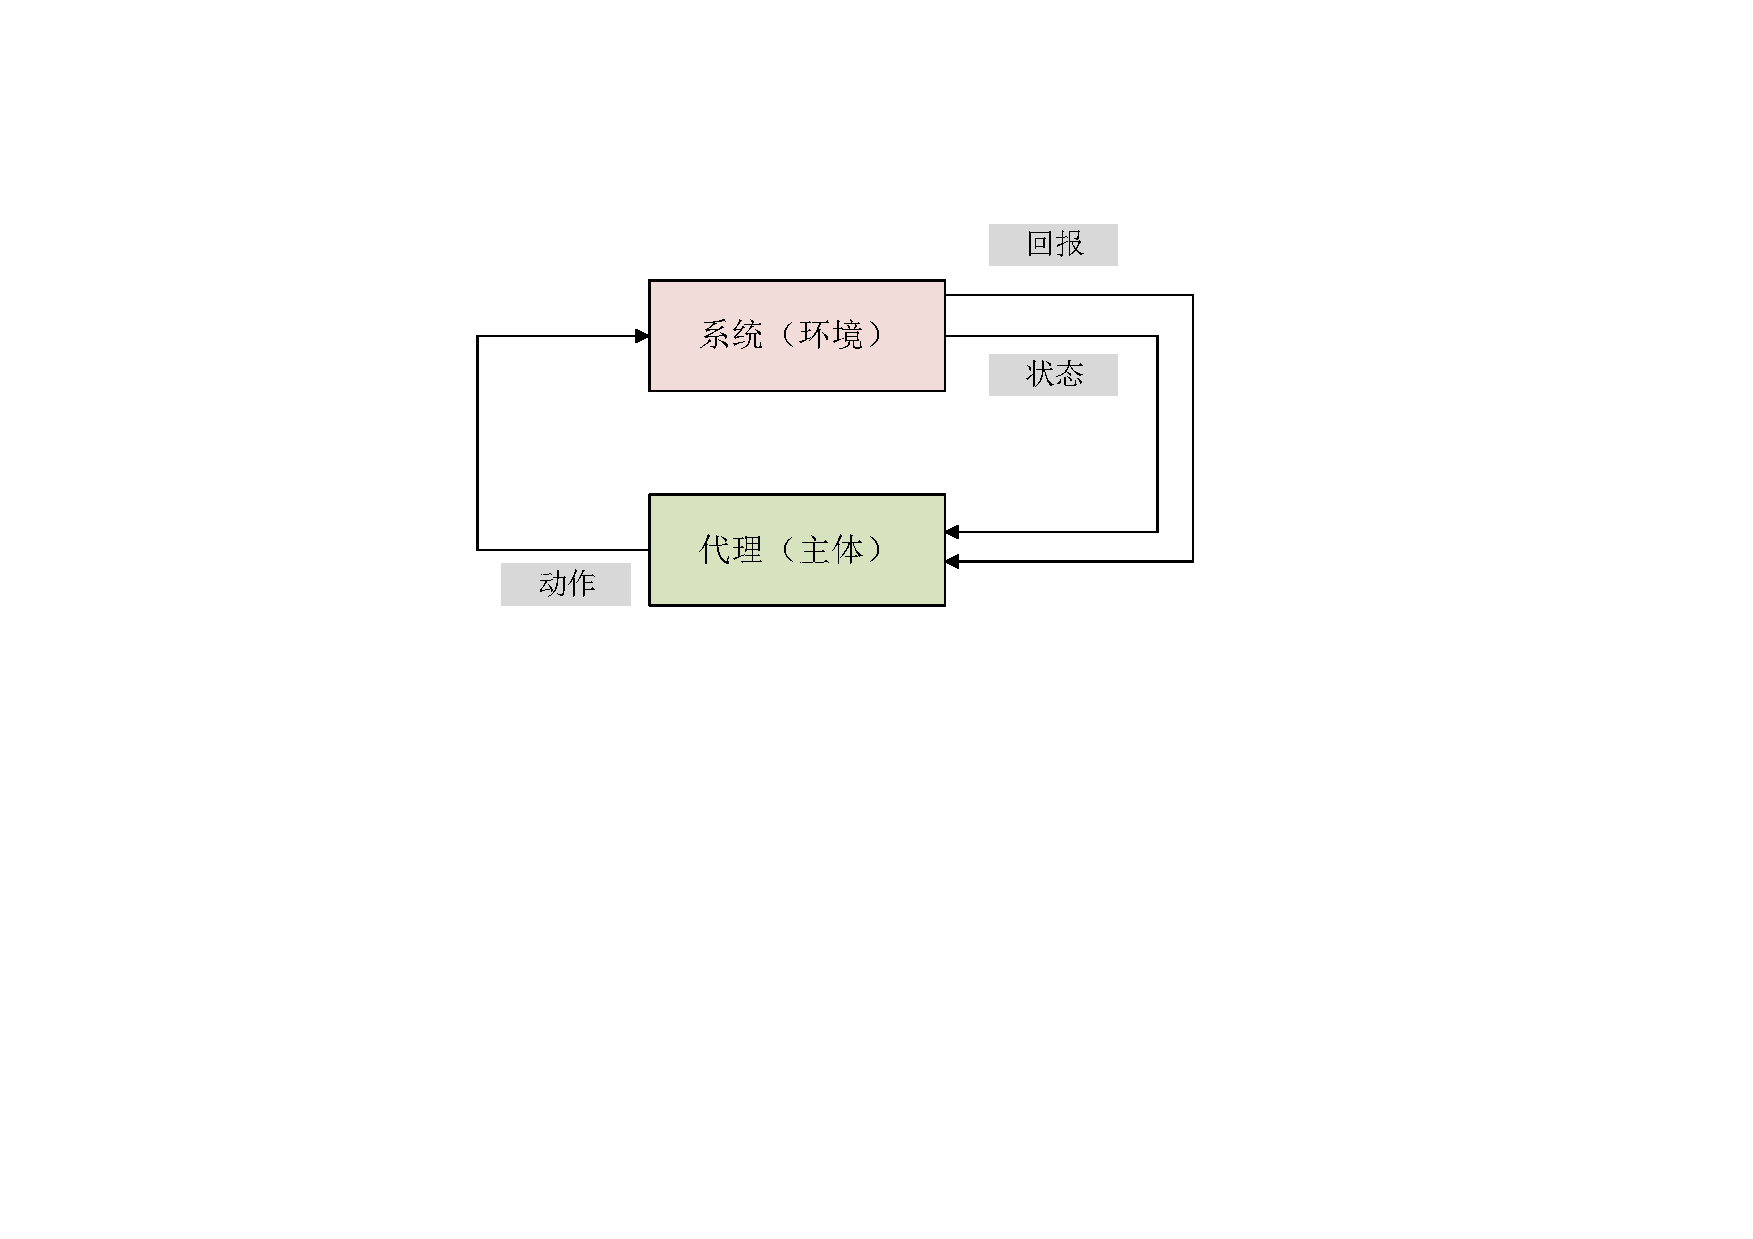
\includegraphics[width=0.4\textwidth]{reinforcement.pdf}}
\caption{基本强化学习过程示意图}
\label{fig:rein}
\end{figure}
图\ref{fig:rein}直观说明了强化学习的典型过程:进行学习操作的主体收到系统的状态以及与上一次状态转换相关的回报函数,之后主体依据历史信息计算出下一步的操作传送给系统。作为回应,系统转换到下一状态并不断重复上述过程。整个问题的目的在于逐渐学习一系列操作来控制系统,从而最大化总的回报函数。强化学习中包含几类不同的问题,将在第\ref{sec:RL}部分中具体叙述,区别主要在于系统返回数据的方式以及不同的性能度量方法。


\subsection{本文工作}

如前所述,本文的目标之一是在过去的十年中对在蜂窝网络领域实施智能解决方案进行广泛的文献回顾,以便管理和发展日益复杂的网络。本文不仅介绍了与SON相关的最新研究成果,而且还对以前的研究进行了涉及RL算法和自动化功能的实现,以提高蜂窝网络的整体性能。
本文的主要贡献是:
\begin{itemize}
  \item 为读者提供有关SON应用于蜂窝网络的文献的广泛综述,以及在实现SON功能时涉及的最流行的ML算法和技术;
  \item 论文的重点是应用于SON的RL算法的学习视角。本文的贡献不是提供SON功能的概述,更多的是为读者提供对实现这些SON功能的最新算法的理解和分类;
  \item 本文还尝试根据各自的SON功能和ML实现对每种算法进行分类;
  \item 本文还提出了基于其应用的学习和技术对不同算法进行分类;
  \item 根据一些SON要求比较不同的ML技术;
  \item 提供关于何时对每个SON功能使用每个ML算法的一般准则;
\end{itemize}

具体内容分为以下几个部分:第\ref{sec:RL}部分介绍强化学习的发展,以及应用较为广泛的算法。第\ref{sec:SON}部分对SON 的发展中出现的问题进行介绍,并分类总结强化学习在各种问题下的应用。第\ref{sec:Compare}部分对比各类算法在解决SON中问题的性能进行分析。\ref{sec:Conclusion}部分进行总结本文涉及的相关内容并展望未来SON发展方向,以及强化学习面临的新型问题。
\section{强化学习}
\label{sec:RL}
%介绍强化学习的定义以及组成部分,包括:策略、奖励函数、估值函数、代理、环境模型等。

%这种方法是基于系统的思想,在这种场景下称为\emph{代理(Agent)},通过代理与周围环境的交互,以获得用于描述当前\emph{系统状态(State)}的信息量用于选择对于当前环境应当做出的\emph{行为(Action)}。与其他学习算法不同的是,强化学习的系统在执行某个行为之后会反馈给代理一个参数,\emph{收益(Reward)} 或者\emph{损失(Loss)}, 用于评估此行为的优劣\cite{Sutton1998}。
%
%一般来讲,强化学习的模型分为以下四个部分:
%\begin{itemize}
%\item \emph{策略(Policy)}:表示代理根据系统当前状态做出的向动作的映射;
%\item \emph{回报函数(Reward function)}:提供了对当前状态的评估,并根据此前采取的行动的结果计算出回报或者损失;
%\item \emph{值函数(Value function)}:维持一些策略回报的均值,来试图找到最大化回报的长期政策;
%\item \emph{环境模型(Environment model)}:决定状态集合以及代理可能采取的行动集合。
%\end{itemize}
%
%由于强化学习算法具有评估每次行为的奖励机制,因此存在\emph{探索(Exploration)}与\emph{利用(Exploitation)}之间的权衡关系,具体表现为代理人必须决定在接下来的迭代过程中,究竟是在系统中探索其他行为,以发现未知行为带来的更高回报,还是保持现有的已知信息,并最大限度地利用当前已知最高回报的行为。
%
%强化学习发展至今,具有广泛应用的算法有以下几种,多臂老虎机(MAB),动态马尔科夫决策过程,Q-学习算法等。其中Q-学习算法是利用Q-函数计算并不断优化,以得到系统的最佳策略。基于Q-学习算法,\cite{Kaelbling1996} 中结合模糊逻辑的相关控制方法,形成一套有效的强化学习算法,称为模糊Q-学习算法。对于上述强化学习算法的具体过程将在第\ref{sec:RL} 部分中详细介绍,此外关于具体算法应用于SON的相关问题,将在接下来的部分分别展开讨论。


这种方法是基于系统的思想,在这种场景下称为\emph{代理(Agent)},通过代理与周围环境的交互,以获得用于描述当前\emph{系统状态(State)}的信息量用于选择对于当前环境应当做出的\emph{动作(Action)}。与其他学习算法不同的是,强化学习的系统在执行某个行为之后会反馈给代理一个参数,\emph{收益(Reward)} 或者\emph{损失(Loss)}, 用于评估此行为的优劣\cite{Sutton1998}。

一般来讲,强化学习的模型分为以下四个部分:
\begin{itemize}
\item \emph{策略(Policy)}:表示代理根据系统当前状态做出的向动作的映射;
\item \emph{回报函数(Reward function)}:提供了对当前状态的评估,并根据此前采取的行动的结果计算出回报或者损失;
\item \emph{值函数(Value function)}:维持一些策略回报的均值,来试图找到最大化回报的长期政策;
\item \emph{环境模型(Environment model)}:决定状态集合以及代理可能采取的行动集合。
\end{itemize}

由于强化学习算法具有评估每次行为的奖励机制,因此存在\emph{探索(Exploration)}与\emph{利用(Exploitation)}之间的权衡关系,具体表现为代理人必须决定在接下来的迭代过程中,究竟是在系统中探索其他行为,以发现未知行为带来的更高回报,还是保持现有的已知信息,并最大限度地利用当前已知最高回报的行为。

强化学习发展至今,具有广泛应用的问题模型有以下两种:多摇臂赌博机(Multi-armed Bandit Problem),有限马尔科夫决策过程(Finite Markov Decision Process)。其中两类模型又包含多种具体模型以及算法思想。下面将给出一些常用模型及其对应算法在蜂窝网络通信中的具体应用,每种算法用一些例子以及具体参考文献加以说明。

%Q- 学习算法是利用Q- 函数计算并不断优化,以得到系统的最佳策略。基于Q-学习算法,\cite{Kaelbling1996} 中结合模糊逻辑的相关控制方法,形成一套有效的强化学习算法,称为模糊Q-学习算法。对于上述强化学习算法的具体过程将在第\ref{sec:RL} 部分中详细介绍,此外关于具体算法应用于SON 的相关问题,将在接下来的部分分别展开讨论。

\subsection{多摇臂赌博机问题(MAB)}
多摇臂赌博机(MAB)问题的实际原型即为一个人在赌场中面对一排(单摇臂)赌博机时,需要决定玩哪一台机器,在每台机器上玩几次,按什么顺序玩这些机器可以让自己赢尽可能多的钱。在这里我们假设每台机器都有其一定的赢钱概率。将这一排单臂赌博机看作一个多摇臂赌博机,就成为了我们所研究的多摇臂赌博机模型。从理论上来定义,MAB问题为由一系列动作决定的资源序列分配问题。在每个时隙,单位资源被分配给一个动作并获得回馈信号,问题目标是最大化获得的总回馈信号值,基本点是选择当前回馈信号最优的项目与选择未来可能有更大回馈信号项目之间的冲突。由此可以看出回馈信号起到两个作用:一是增加总回报,二是提供信息以推测各摇臂的性能表现。MAB问题目前已经在蜂窝网络通信问题中得到了应用,例如。
\subsubsection{随机性多摇臂赌博机(Stochastic Bandit)}
随机性MAB问题中,每个摇臂上的回馈信号都服从一个未知的统计概率分布,相当于每个摇臂的性能是确定的。

$\epsilon$-greedy 随机选取非估计最优; UCB联合考虑估计值与估计的不确定度;基于此思想考虑变形问题:不稳定;休眠;相关性;


\cite{Wang2017}利用摇臂间具有相关性以及贝叶斯思想来自动优化室内小基站的信号发射功率;\cite{Shen2017}中利用随机性MAB算法解决小基站切换问题;\cite{Simsek2015a}中利用UCB算法解决异构网中的干扰控制问题。

\subsubsection{对抗性多摇臂赌博机(Adversarial Bandit)}
对抗性MAB与随机性MAB不同,回到最初对MAB实际情况的说明,对抗性MAB相当于是在一个有作弊手段的赌场里,店家可以操作赌博机,在每个时隙可以任意设定回馈信号的值来满足自身利益,每次调整回馈信号可能依赖也可能独立于以往的决策动作。
\cite{Maghsudi2017}解决小基站网络中用户关联问题; \cite{Shen2016}异构网中用户的移动性接入问题。

\subsubsection{有情境赌博机(Contextual Bandit)}
\cite{Simsek2015a}

\subsubsection{有状态赌博机(Markovian Bandit)}
\cite{Sun2017}中利用用户行为特征来优化异构网中基站与用户的关联问题; \cite{Tekin2011}解决机会频谱接入问题。
%常见的MAB算法分类,以及我们组所做相关工作。

%\subsection{Q-学习算法}

%重点介绍,Q-学习方法应用较多,基于此方法添加模糊逻辑,形成的模糊Q-学习方法在通信中的应用较为广泛。

\subsection{有限马尔科夫决策过程}
MDP问题是满足马尔科夫性质的一类强化学习问题。一个特定的马尔科夫决策过程由状态、动作集与环境的一步动态定义。由于对状态及策略的具体建模,MDP可以在普遍程度上刻画大部分的强化学习问题。在马尔科夫决策问题中一般依据贝尔曼方程,通过求解最优值函数来获得最优策略。传统的解决方法一般利用动态规划,但对于状态空间较大的情况复杂度较高不易处理。

\subsubsection{Q-learning}
强化学习中较常用的估计值函数的方法为Q-学习算法,利用产生的Q函数估计序列逐渐收敛于最优值。
 \cite{Simsek2015}解决异构网中基站间干扰控制问题; \cite{Ghadimi2017}解决蜂窝网络中下行链路的功率控制问题。

\subsubsection{Fuzzy Q-learning}
基于Q-学习方法添加模糊逻辑,形成的模糊Q-学习方法在通信中的应用也很广泛。
\cite{Munoz2013}解决企业小基站网络中负载均衡问题。



\section{自组织网络应用发展}
\label{sec:SON}
%本文的重点章节,各个技术应用的问题介绍清楚,分类所有的强化学习的文章
LTE的部署对SON的推进,涉及到若干问题及其解决方案。
下列各种应用对应的实际问题可以参考\cite{Klaine2017}中Introduction部分的分类。

5G 系统采用了复杂的无线传输技术和无线网络架构,使得网络管理远远比与现有网络复杂,网络深度智能化是保证 5G 网络性能的迫切需要。因此,自组织网络将成为5G的重要技术。

5G 将是融合、协同的多制式共存的异构网络。从技术上看,将存在多层、多无线接入技术的共存,导致网络结构非常复杂,各种无线接入技术内部和各种覆盖能力的网络节点之间的关系错综复杂,网络的部署、运营、维护将成为一个极具挑战性的工作。为了降低网络部署、运营维护复杂度和成本,提高网络运维质量,未来 5G 网络应该能支持更智能的、统一的 SON 功能,能统一实现多种无线接入技术、覆盖层次的联合自配置、自优化、自愈合。目前,针对 LTE 、 LTE-A 以及 UMTS 、WiFi 的 SON 技术发展已经比较完善,逐渐开始在新部署的网络中应用。但现有的 SON 技术都是面向各自网络,从各自网络的角度出发进行独立的自部署和自配置、自优化和自愈合,不能支持多网络之间的协同。因此,需要研究支持协同异构网络的 SON 技术,如支持在异构网络中的基于无线回传的节点自配置技术,异系统环境下的自优化技术,如协同无线传输参数优化、协同移动性优化技术,协同能效优化技术,协同接纳控制优化技术等,以及异系统下的协同网络故障检测和定位,从而实现自愈合功能。

5G 将采用超密集的异构网络节点部署方式,在宏站的覆盖范围内部署大量的低功率节点,并且存在大量的未经规划的节点,因此,在网络拓扑、干扰场景、负载分布、部署方式、移动性方面都将表现出与现有无线网络明显不同之处,网络节点的自动配置和维护将成为运营商面临的重要挑战。比如,邻区关系由于低功率节点的随机部署远比现有系统复杂,需要发展面向随机部署、超密集网络场景的新的自动邻区关系技术,以支持网络节点即插即用的自配置功能;由于可能存在多个主要的干扰源,以及由于用户移动性、低功率节点的随机开启何关闭等导致的干扰源的随机、大范围变化,使得干扰协调技术的优化更为困难;由于业务等随时间和空间的动态变化,使得网络部署应该适应这些动态变化,因此,应该对网络动态部署技术进行优化,如小站的动态与半静态开启和关闭的优化、无线资源调配的优化 ;为了保证移动平滑性,必须通过双连接等形式避免频繁切换和对切换目标小区进行优化选择;由于无线回传网络结构复杂,规模庞大,也需要自组织网络功能以实现回传网络的智能化。


\subsection{自配置应用}
\label{sec:self-configuration}

在SON中,自配置是指自动配置当前网络中,如微基站,中继站,宏基站等所有设备参数的过程。此外,若当前网络系统已经开始运行,又有新网络节点引入以及设置,或者网络从故障中重新启动,此时自配置包括站点位置选择、硬件配置标准化以及每个新网络节点的准备、安装、鉴权和认证,基本涵盖了将一个新节点纳入网络中运行的全部过程 \cite{Aliu2013}。针对SON中出现的不同类型问题,\cite{Wainio2016}提出了一种通用框架,在自配置的角度,该框架提供实现网络自组织的所需的一些基本步骤,首先在部署之前,基站已经配置基本的操作参数,这些参数对于各种实际应用场景是不变的,因此不需要再次部署。其次,第二阶段的配置包括扫描并确定基站的相邻基站,建立起邻基站列表(Neighbour Cell List, NCL)。最后阶段是基于现有网络拓扑,对新部署的基站后的网络进行参数调整。与该方法不同的是 \cite{Hu2010}文中提出的部署新基站的方式为感知并选中一个相邻基站进行所必须的参数请求以及下载。因此,无论哪种方法,自配置的基本应用包括部分 1)配置基站基本操作参数,2)探测邻小区并配置NCL参数,3)调整网络拓扑匹配当前新添加的基站。

为了实现自配置,目前应用的学习算法不仅可以配置基本的操作参数而且可以发现邻域基站并初始化。由于异构网络的复杂度增加,以及基站的功能日渐丰富,造成自配置阶段需要处理的参数也大量增加,而且参数之间的耦合性也是系统运维人员需要考虑的重要因素。根据上述的问题以及解决方案的主要步骤,在接下来的用例中讨论强化学习解决方案。

\subsubsection{操作参数配置}

网络自配置的第一阶段是关于基站基本参数的初始化操作,包括IP地址、网关、小区标识(Cell IDentity,CID)、物理小区标识(Physical Cell Identity,PCI)等参数。

Imran等人在\cite{Imran2013a}提出用于描述蜂窝网系统中主要的关键性能指标的框架,以及此后出现多种将系统的整体规划与分析模型相结合的方案,均用于解决多目标优化问题,以确定最佳的小区规划参数,例如基站位置、扇区数、天线高度、方位角、传输功率和频率重用因数等。

Hu等人在\cite{Hu2010}提出自配置的辅助解决方案,用于网络中部署新的基站。文章指出新的基站应获取自身的IP地址和操作、管理和维护中心。该过程可以通过动态主机配置协议(Dynamic Host Configuration Protocol,DHCP)、引导协议(BOOTstrap Protocol,BOOTP)或通过使用Internet组管理协议(Internet Group Management Protocol,IGMP)进行多项转换来完成。之后,新基站搜索附近的相邻小区,并获取无线电参数并继续其他的操作。

从智能的角度来看,\cite{Wainio2016}和\cite{Hu2010}的解决方案并不适用于学习算法,因为它们都依赖于预先配置的参数以及其他相邻基站的信息。Peng等人在\cite{Peng2013}给出智能算法解决在异构 LTE 网络中配置PCI和覆盖率等相关参数的思路。在PCI配置方面,文章中提出一种基于分组的算法,先将PCI资源与基站划分为多个子集,然后将每个站点分配到特定的子集中,通过基站之间的PCI参数的自主分配,在网络中实现最大化PCI复用距离,并同时避免了多路复用干扰。

\subsubsection{NCL参数配置}

当系统中有新基站添加进入时,它应当感知相邻一定范围内的其他基站,并建立起通信连接,从而实现网络的基本功能,例如切换(HandOver,HO)。而NCL则是蜂窝网系统基于当前所有基站的统计信息,对新添加基站的进行管理的数据库列表。

5G技术的逐步完善,给不同系统间的基站切换带来更为复杂的挑战。为了完成UMTS、CDMA以及LTE等不同系统之间的自由切换,以实现无线通信的平滑过渡,基站在维护NCL时采用更为先进的模式。新的模式是通过自动邻区关系(ANR)功能实现的,\cite{3gpp.32.511} 提出解决不同系统之间用户切换的策略:预规划黑白列表,初始化次优化临区列表,甚至初始化空白临区列表等。对NCL的配置依赖于两种功能的实现,一方面是必须感知到新部署基站的加入,并向该基站发送所需要的NCL信息,另一方面必须将新部署基站信息添加到相邻基站的NCL中。

现有的文章较多注重于感知新部署基站加入时的部署问题研究,如\cite{Lee2014},\cite{Kim2010},但也有一些作者侧重于研究后一种问题。如\cite{Wainio2016}中,作者提出现利用现有的基站周期性地扫描周围环境,进行NCL信息交换,在扫描过程中若出现新的基站则添加到现有网络中。大部分作者提出的解决方案都依赖于使用反馈控制器来执行NCL配置,没有考虑更为智能化的配置方法。

Li等人在\cite{Li2007}中提出两种不同配置方案,第一种解决方案基于基站之间的物理距离,通过判断原有基站是否在新部署基站的给定半径的范围内,若在该范围内,则将该基站添加到新部署基站的NCL中。第二种方案不仅评估相邻基站的距离,而且引入天线参数,并由小区重叠的情况确定是否添加该NCL项。


\subsubsection{无线电参数配置}
在得到NCL信息之后,基站必须配置其余的无线电参数,包括小区标识,基站功率设置,切换设置参数(如滞后时间和触发时间),随机接入信道参数导频功率,分段资源分配,以及其他相关的配置新基站的无线资源管理参数。

传统的无线电参数配置方式是根据从其邻居基站收集到的测量值和数据来调整,例如在\cite{Sanneck2010}中,作者提出一种LTE基站的自配置架构,这种架构下配置基站参数是通过动态分配基站参数的子集实现的。文章中提出动态无线电配置功能 (DRCF),评估基站的邻居覆盖区域,以确定新基站的最佳参数,形成小区群并提供跟踪区域码(TAC),减少配置复杂度。

此外,在无线电参数配置中应用强化学习算法也是较为普遍的解决方案,在\cite{Razavi2010}中,Razavi提出可以通过学习算法来配置天线下倾角度,以实现调整基站的覆盖范围和容量。作者在文章具体分析了LTE网络系统的场景下三种不同的模糊Q学习算法,并且从学习速度和收敛性方面做出比较。第一种情况在每个时隙中仅研究一个小区的参数配置情况,第二种场景中同时研究所有的小区,第三种场景是将所有的小区分成若干个簇,每个时隙只允许一个小区簇进行更新。结果表明所有的方法都能够学习到最佳天线下倾角,但前两种方法的弊端分别是收敛速度过慢,以及复杂度过高。所以使用小区簇的方式可以达到学习收敛速度与复杂度的折中。

更进一步的工作在\cite{Razavi2010a}中展示,文章提出了分布式FQL算法, 以便在LTE网络场景中配置天线的下倾角度。此外,作者从频谱效率的角度对算法性能进行了评价, 并将算法与模糊规则 (ELF) 的学习进行了比较。另外一种采用FQL 概念的工作由Islam 在\cite{Islam2012}中提出。在尝试利用调整下倾角度的方法解决参数配置问题的基础上,文章还考虑了热噪声和接收机噪声两个噪声源,将结果与标准模糊规则进行了对比。

表格中列出了自配置用例及其各自的学习算法的应用。


\subsection{自优化应用}
\label{sec:self-optimization}
移动网络是动态变化的,包括不断地部署新站地址,扩充当前网络容量,调整参数以适应本地业务量和环境条件。在无线自组织网络中,自优化的概念被定义为不断监视网络极其环境参数的函数,并更新相应的参数,以保证网络尽可能高效的运行\cite{Aliu2013}。网络优化是连续的闭环处理过程,包括周期性的性能评估,参数的优化以及优化后参数的重新部署。初始化阶段自配置得到的参数在后期不再适用,需要进行优化以提升网络性能。由于网络中需要优化的参数规模较大,耦合性强,复杂度较高,????

优化过程中所需要的输入数据可以通过不同的途径获得,例如运行和维护(Operation and management)性能测量,追踪主要接口(例如:Uu、Iub和Iu等)以及联合位置信息的接口测量数据的路测技术。网络运营商在网络运行的过程中收集了大量的数据,进而为优化网络的智能解决方案应用提供训练数据支持。利用用户设备和基站收集的测量值和性能指标,结合强化学习算法进行自动调整网络设置是一种可行的自优化方案。基于\cite{3gpp.36.902}中定义的用例以及本文所引用的相关文献,自优化的应用在以下部分进行描述。

\subsubsection{回程线路优化}

回程线路(Backhaul)是蜂窝网络系统中较为重要的概念,它表示基站与基站控制器之间的链接,是基站接入核心网的实现途径。现行的蜂窝网络系统仅考虑用户与基站之间的信号连接质量,但由于系统规模的不断扩张,这种方法无法解决不同类型的数据在更广泛的应用程序的可靠性问题。而回程线路可以改善用户和核心网络之间的连接,基于此的网络优化设计面临的问题在不同的文献中以不同方式描述,例如服务质量(QoS),用户体验质量(QoE),拥塞控制以及网络拓扑管理等。
%\cite{Wainio2016} 以及\cite{Chernov2014} 中提出。

现有文献中提到的解决方案设计的范围较为广泛,例如\cite{Wainio2016}和\cite{Chen2015}在文章中提出的回程线路优化方案涉及到灵活的QoS方案,拥塞控制机制,负载均衡以及调度均衡等问题。而另外一种回程线路优化方案是使用强化学习中较为经典的Q-学习算法,\cite{Jaber2015}\cite{Jaber2016a}\cite{Jaber2016c}将用户用不同类型的需求来描述,比如对容量、延迟等参数的要求。而回程线路由分布各不相同的基站提供,若搜索到的回程线路的参数满足该用户需求,则建立起回程线路与用户的连接;否则继续搜索满足要求的基站来提供回程线路。文章结论表明提出的Q-学习算法可以为用户在一定范围内牺牲总的吞吐量带来较大的服务质量的提升。

从引入回程线路的作用来看,未来网络的优化必然考虑这一因素,但现在并未普及。因此未来研究方向可以从这一领域进行探索。

\subsubsection{缓存}

缓存(Caching)在网络中的重要性随着多媒体以及流媒体服务的流行日益增加。由于智能手机的普及,移动网络的通信量呈几何式增长,而数据传输的速率和滞后时间的要求在某些业务下更为严格。


\subsubsection{容量}
\subsubsection{移动性管理}
\subsubsection{切换参数优化}
\subsubsection{负载均衡}
\subsubsection{资源优化}



\subsection{自动愈合应用}

在自组织网络中,自愈合可以定义为一种自发执行的行为,它可以保证网络的正常运行,以及防止破坏性问题的出现。具体的功能不仅包括解决坑你发生的故障,而且应当自动执行故障检测、诊断、以及触发相应的纠正机制,在网络异常发生之前采取必要的措施。目前网络故障解决方案依靠人工干预以及反应性方法,即只有在网络中出现故障导致系统运行产生错误后才会触发愈合过程,这种方式会降低蜂窝网的服务质量。从学习算法的角度来考虑这个问题则具有一定的挑战性。学习算法试图预测故障出现时的多种特征,依赖于先前搜集到的大量数据,以便建立相应的数学模型。某些情况下可以很容易的对得到的数据类型进行标记,例如故障分类。但对其他类型的数据进行标记,例如系统停运时,有些变量并没有发生明显的变化,这种情况下的故障与数据之间的联系就并不关键。



执行网络运行和阻止出现突发情况,包括必要的软件和硬件的更新或替换。
\subsubsection{故障检测}
\subsubsection{故障分类}
\subsubsection{服务中断管理}

\section{自组织网络中的强化学习算法}
\label{sec:Compare}
对比各类算法在自组织网络中解决问题的性能分析,包括稳定性,时效性,准确度,收敛时间,复杂度等。
依据 \cite{Klaine2017} Section  VI中提到的性能参数对上一部分中提及参考文献所涉及的技术进行横向对比。

\section{未来发展方向}
\label{sec:Conclusion}
从自组织网络不同应用方向出发,分析现存的问题,并提出未来解决方法以及相关技术的发展方向。

\section{结论}


\bibliographystyle{IEEEtran}

\bibliography{SON,RL}
\end{document}
